\subsection{Diagrammes des cas d'utilisation}
    \subsubsection{Cas général}
    \paragraph{}
    \begin{figure}
        \centering
        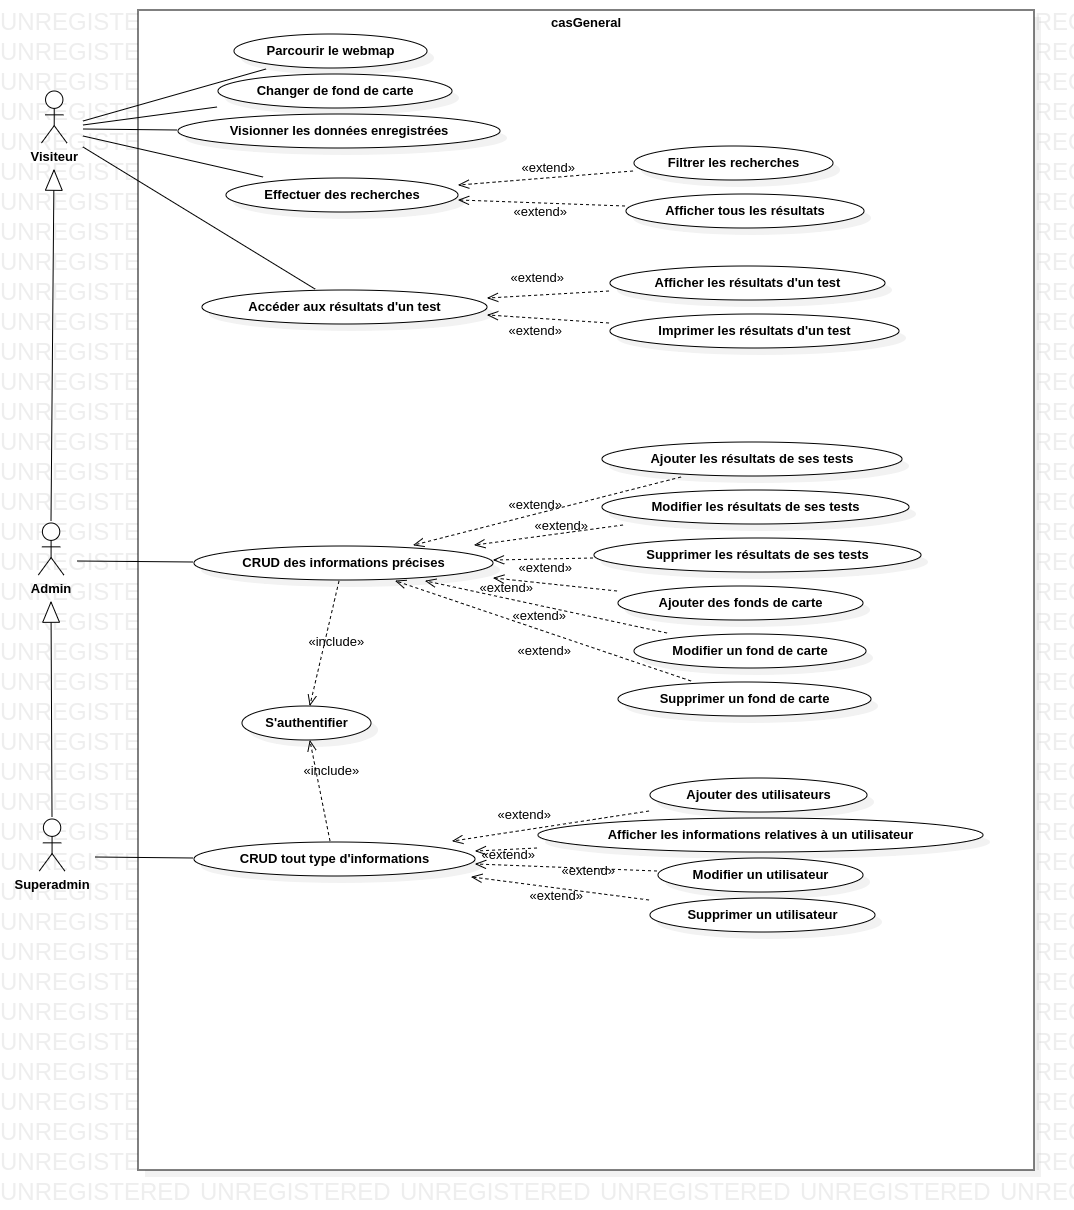
\includegraphics[width=1\textwidth]{images/Analyse_des_besoins/casGeneral.png}
        \caption{Diagramme des cas d'utilisation général}
    \end{figure}
    \par 
    Trois niveaux d'acteurs sont à considérer au sein du système: un visiteur, 
    un administrateur et un super administrateur. La hiérarchisation permet que 
    chaque niveau ait accès aux droits du niveau immédiatement inférieur. 
    De ce fait, un super administrateur est également un administrateur et 
    un visiteur en plus de son niveau direct. \par 
Pour commencer, le visiteur a des droits d'accès très restreints: \par 
\begin{itemize}
    \item Parcourir le webmap: Le visiteur peut voir l'ensemble des informations 
    géotechniques disponibles sur la carte.
    \item Changer de fond de carte: Afin de mieux illustrer le contexte marquant 
    l'intérêt du visiteur, une variété de fonds de carte est accessible sur le site. 
    Ainsi, l'utilisateur peut puiser dans le champs de choix qui lui sont proposés.
    \item Visionner les données enregistrées: En cliquant sur une légende précise, 
    le visiteur peut voir les données qui ont été préalablement enregistrées dans la base de données.
    \item Effectuer des recherches: Deux options s'offrent aux utilisateurs. Ces derniers 
    peuvent afficher tous les résultats au cours de la rechercherche, ou encore ils peuvent 
    se fixer des filtres capables de mieux limiter les plages des résultats.
    \item Accéder aux résultats d'un test: Une fois les résultats obtenus, le visiteur 
    peut soit simplement les afficher, soit les imprimer.
\end{itemize}

\paragraph{}
De son côté, l'\textbf{administrateur} s'occupe de la gestion des informations au sein de la base 
de données. En plus des droits de visiteur, ce type d'utilisateur peut:
\begin{itemize}
    \item Ajouter des informations géotechniques: L'admin peut ajouter des informations 
    dans la bdd, qui sont reflétées sur la carte. 
    \item Modifier les informations qu'il avait préalablement enregistrées: Il ne peut 
    modifier que les informations qu'il avait lui-même ajoutées.
    \item Supprimer les informations qu'il avait préalablement enregistrées: Tout comme il 
    en est pour la modification, il ne peut supprimer que les informations qu'il avait lui-même ajoutées.
    \item Ajouter un fond de carte
    \item Supprimer un fond de carte
\end{itemize}

\par 
Évidemment, aucune de ces actions ne saura avoir lieu tant que l'administrateur ne s'est pas authentifié.

En dernier lieu, le super administrateur joue surtout un rôle de gestionnaire en ressources 
humaines. Une fois authentifié, en plus des droits d'accès d'un simple administrateur, 
cet utiliateur peut:
\begin{itemize}
    \item Ajouter des utilisateurs
    \item Modifier les utilisateurs
    \item Afficher les informations relatives aux différents utilisateurs, pouvant 
    ainsi retracer toutes les actions posées par un utilisateur du système.
    \item Supprimer ou désactiver un utilisateur: La différence se fait remarquer 
    par le fait que le super admin peut supprimer complètement un utilisateur ainsi 
    que toutes les informations y relatives ou simplement désactiver le compte d'un 
    utilisateur sans, pour autant, éliminer ses données.
\end{itemize}

\subsubsection{Parcourir le Webmap}
    \paragraph{}
    \begin{figure}
        \centering
        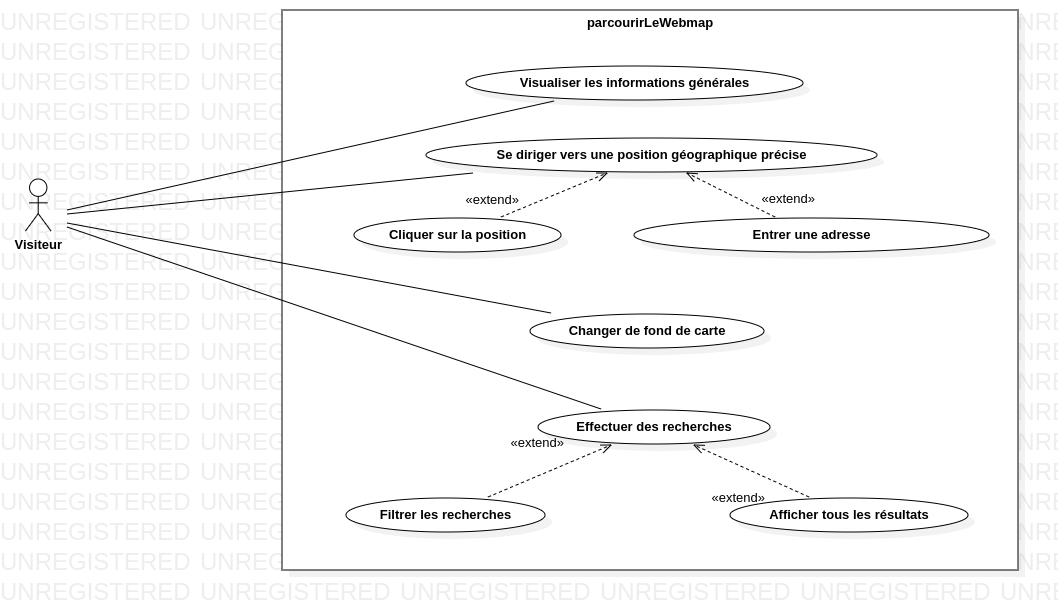
\includegraphics[width=1\textwidth]{images/Analyse_des_besoins/parcourirLeWeb.png}
        \caption{Diagramme du parcours du webmap}
    \end{figure}
\par 
Tout individu, concernés ou pas, par les informations fournies par 
le webmap peut parcourir l'application. Pour ce faire, aucune authentification 
n'est nécessaire au préalable. Lorsqu'un visiteur accède au site, il peut donc:
\begin{itemize}
    \item \textbf{Visualiser les informations générales:}
    Les informations sont disponibles sur une carte pouvant être interprétés
    par un particulier. Elles sont étiquetées sur les points géographiques respectives.
    De ce fait, il peut sélectionner une étiquette particulière afin d'avoir 
    accès à ces données, lui permettant de 
    \begin{itemize}
        \item Visualiser le fichier pdf
        \item Télécharger ce fichier
    \end{itemize}
    \par 
    À première vue, le visiteur ne voit que la carte remplie de 
    "pin[MPOKO JWENN TERME FRANCAIS A]" colorés relatifs à une légende 
    explicite pour la compréhension du visiteur. En plus des légendes, une liste 
    de wigdets facilitant la navigation de l'utilisateur.
    \item \textbf{Accéder à une position géographique précise}
    Toutes les informations étant disponibles, le visiteur peut choisir 
    de visualiser les données relatives à une position bien définies. Pour y accéder, il 
    peut:
    \begin{itemize}
        \item Cliquer directement sur la position géographique
        \item Entrer une adresse dans le champs y frelatif
    \end{itemize}
    \item \textbf{Changer de fond de carte}
    Chaque individu visite ce webmap dans un contexte personnel. Par 
    ailleurs, il peut changer le fond de la carte en fonction de 
    ses besoins. Ces images peuvent varier d'un point de vue hydraulique
    à un point de vue magmatique en passant par tous les fonds mis 
    à la disposition de l'utilisateur par les institutions.
    \item \textbf{Effectuer des recherches relatives aux essais}
    Grand nombre d'essais sont enregistrés sur la carte. Pour faciliter 
    la navigation, une possibilité de recherche est offerte. Dans ce cas,
    il peut donc:
    \begin{itemize}
        \item Afficher tous les résultats
        \item Filtrer les recherches 
    \end{itemize}
\end{itemize}

\subsubsection{Manipulation des données de la base}
    \paragraph{}
    \begin{figure}
        \centering
        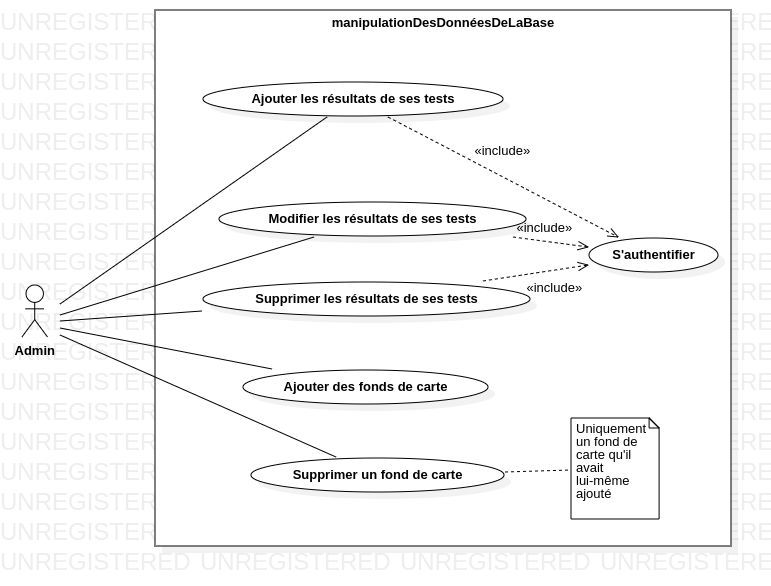
\includegraphics[width=1\textwidth]{images/Analyse_des_besoins/manipulationDesDonneesDeLaBase.png}
        \caption{Diagramme de la manipulation des données de la base}
    \end{figure}
    \par 
    Avant même que les données puissent être disponibles et interprétables 
    par un utilisateur, il faut qu'elles soient intégrées et manipulées continuellement. Le 
    seul utilisateur ayant habilité à faire de telles 
    actions est l'administrateur. Néanmoins, il ne peut manipuler que les informations 
    qu'il a lui-même insérées dans la base de données. Ces dernières étant sensibles, L'admin 
    doit s'authentifier avant d'avoir des droits d'accès à toute sorte de manipulation.

    \subsection{Diagramme de classes}
    \paragraph{}
    Il s'agit du diagramme le plus important dans le cadre 
    d'une modélisation orientée objet. Grâce à lui, le concepteur peut 
    représenter la structure interne du travail à réaliser, lui 
    permettant de trouver un meilleur terrain d'entente avec le client.
    \par 
    Trois grandes classes sont donc implémentées:
    \begin{itemize}
        \item Utilisateur
        \item Institution
        \item Essai 
    \end{itemize}
    \par 
    [TO BE CONTINUED]